\documentclass[]{article}
\usepackage{lmodern}
\usepackage{amssymb,amsmath}
\usepackage{ifxetex,ifluatex}
\usepackage{fixltx2e} % provides \textsubscript
\ifnum 0\ifxetex 1\fi\ifluatex 1\fi=0 % if pdftex
  \usepackage[T1]{fontenc}
  \usepackage[utf8]{inputenc}
\else % if luatex or xelatex
  \ifxetex
    \usepackage{mathspec}
  \else
    \usepackage{fontspec}
  \fi
  \defaultfontfeatures{Ligatures=TeX,Scale=MatchLowercase}
\fi
% use upquote if available, for straight quotes in verbatim environments
\IfFileExists{upquote.sty}{\usepackage{upquote}}{}
% use microtype if available
\IfFileExists{microtype.sty}{%
\usepackage{microtype}
\UseMicrotypeSet[protrusion]{basicmath} % disable protrusion for tt fonts
}{}
\usepackage[margin=1in]{geometry}
\usepackage{hyperref}
\hypersetup{unicode=true,
            pdftitle={Music and Memory},
            pdfauthor={Lizhou Fan, Kaixin Wang and Huizi Yu},
            pdfborder={0 0 0},
            breaklinks=true}
\urlstyle{same}  % don't use monospace font for urls
\usepackage{longtable,booktabs}
\usepackage{graphicx,grffile}
\makeatletter
\def\maxwidth{\ifdim\Gin@nat@width>\linewidth\linewidth\else\Gin@nat@width\fi}
\def\maxheight{\ifdim\Gin@nat@height>\textheight\textheight\else\Gin@nat@height\fi}
\makeatother
% Scale images if necessary, so that they will not overflow the page
% margins by default, and it is still possible to overwrite the defaults
% using explicit options in \includegraphics[width, height, ...]{}
\setkeys{Gin}{width=\maxwidth,height=\maxheight,keepaspectratio}
\IfFileExists{parskip.sty}{%
\usepackage{parskip}
}{% else
\setlength{\parindent}{0pt}
\setlength{\parskip}{6pt plus 2pt minus 1pt}
}
\setlength{\emergencystretch}{3em}  % prevent overfull lines
\providecommand{\tightlist}{%
  \setlength{\itemsep}{0pt}\setlength{\parskip}{0pt}}
\setcounter{secnumdepth}{0}
% Redefines (sub)paragraphs to behave more like sections
\ifx\paragraph\undefined\else
\let\oldparagraph\paragraph
\renewcommand{\paragraph}[1]{\oldparagraph{#1}\mbox{}}
\fi
\ifx\subparagraph\undefined\else
\let\oldsubparagraph\subparagraph
\renewcommand{\subparagraph}[1]{\oldsubparagraph{#1}\mbox{}}
\fi

%%% Use protect on footnotes to avoid problems with footnotes in titles
\let\rmarkdownfootnote\footnote%
\def\footnote{\protect\rmarkdownfootnote}

%%% Change title format to be more compact
\usepackage{titling}

% Create subtitle command for use in maketitle
\newcommand{\subtitle}[1]{
  \posttitle{
    \begin{center}\large#1\end{center}
    }
}

\setlength{\droptitle}{-2em}

  \title{Music and Memory}
    \pretitle{\vspace{\droptitle}\centering\huge}
  \posttitle{\par}
  \subtitle{The Island Research Project - Statistics 101B}
  \author{Lizhou Fan, Kaixin Wang and Huizi Yu}
    \preauthor{\centering\large\emph}
  \postauthor{\par}
      \predate{\centering\large\emph}
  \postdate{\par}
    \date{Spring 2019}

\usepackage{float} \floatplacement{figure}{H} \usepackage{lscape}

\begin{document}
\maketitle

\tableofcontents
\newpage

\section{Abstract}\label{abstract}

We have all heard about the saying that music can help improve one's
memory. Based on the fact that we have access to different types of
musical treatments and memory tests, the goal of this research project
is to find whether there is an effect of music on islander's
memorization ability, and which type of music has the most significant
improvement on human's memorization capability. The research is
conducted using the open platform \texttt{The\ Island}\footnote{\href{http://island.maths.uq.edu.au}{\texttt{The\ Island:\ http://island.maths.uq.edu.au}}}.

\section{Introduction}\label{introduction}

According to an annual report produced by the Administration for
Community Living, about one in every seven Americans is over the age of
65 in 2017, and the proportion will swell to one in five by 2040. Old
age is accompanied by declines in mental domains such as processing
speed, reasoning, memory and executive functions (Ian J. Deary, 2009).
As America along with the rest of the world enters an aging society,
there is a growing interest in identifying factors that can alleviate
age-associated cognitive decline.

It has been suggested by some researches (Cirigliano, 2013; Michael,
David, Gerald, \& Volker, 2014) that the temporal pattern structure in
music can enhance cognition and memory retention. This effect appears to
be especially significant for people with cognitive
deterioration/impairment. Such theory has been put to practice by
organizations such as MUSIC AND MEMORY, a non-profit that brings
personalized music playlists to elders in nursing homes. They claim that
`` Music is the most `fast-acting'non-drug approach to improving the
lives of all persons with dementia, Parkinson's, depression and other
behavioural challenges'' (2017 Impact Report, pg 1).

Another interest of substantive researchers is the effect of different
genre of music on memory and cognition. There is a considerable amount
of publication dedicated to investigating the effect of Classical music
on performance and memory retention. Rausher, Shaw and Ky (1993) found
that listening to classical music improved intelligence and memory (the
``Mozart Effect'') and a British radio station specialised in western
classical music was shown to help listeners relax and improve brain
efficiency (Blanchard, 1979). Other studies compared different genres of
music and concluded fast-paced music such as Rap and Heavy Metal may
distract cognitive effects and lead to poorer performance (Dibben \&
Williamson, 2007; Smith \& Morris, 1977).

Due to music's accessibility as well as its universal presence, our
study is interested in testing whether there is theoretical support for
the uses of music as a means for memory improvement. We propose that
listening to music will lead to a statistically significant increase in
the memory test score. For this study, we apply four genres of music
(Country, Classical, Dance, Heavy Metal) as treatment variables and a
control variable (No Music).

In this experiment, our goal is to:

\begin{enumerate}
\def\labelenumi{(\arabic{enumi})}
\tightlist
\item
  test if music is a valid treatment for increasing memory performance;
\item
  find the best genre of music that leads to said improvement.
\end{enumerate}

\section{Experiment}\label{experiment}

\subsection{Participants}\label{participants}

We chose the virtual participants from the online resource the Island.
We found that female who age 65 or older are most susceptible to
cognitive impairment and are outperformed by men (in the same age group)
in fields of visuospatial, verbal processing, semantic and episodic
memory (Laws, K. R. 2016). Because memory retention differs in
individual (M. Karl Healey 2014), and in time of the day (A. D.
Baddeley, 2007), we use Latin Square to block by individual subject and
time of the day. In order to increase power as well as our error degrees
of freedom, we repeated this 5*5 Latin Square five times. This resulted
in our necessary sample size of 25 participants. Moreover, studies have
shown that cognitive impairment and dementia are are predicted to
increase proportionately more in developing regions, thus indicating a
potential association between the region of residence and cognitive
performance (WHO, 2013). We decide to hold this factor constant and
choose participants from the Town Macondo, where the population of
senior citizens is the largest. In order to obtain the 25 participants,
we went to the 64 neighbourhoods of Macondo and request consent from
female participants age 65 to 89.

\subsection{Design}\label{design}

The design that we have chosen to use in this project is 5 x 5 Latin
Square with five replicates.

\textbf{Model}:

\[y_{ijk} = \mu + \alpha_{i} + \beta_{j} + \gamma_{k} + \epsilon_{ijk},\ where\  i, j, k = 1, 2, 3, 4, 5\]

\begin{figure}
\centering
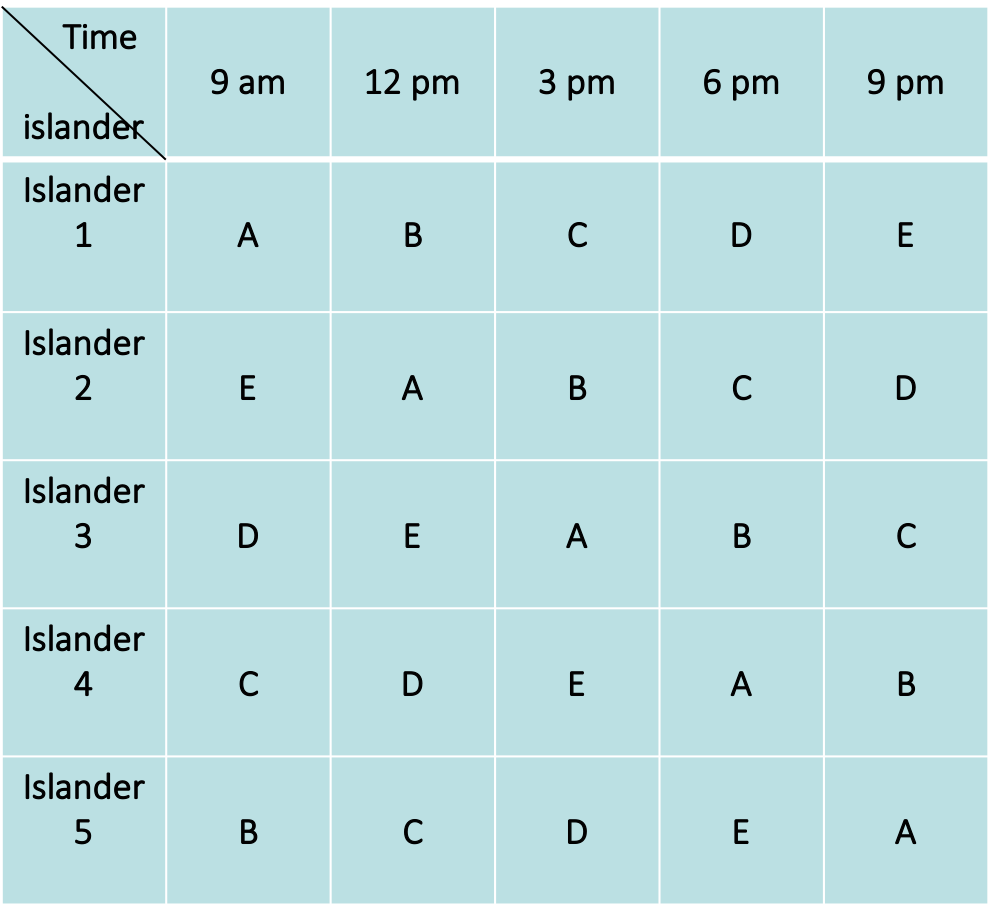
\includegraphics[width=0.80000\textwidth]{Square.png}
\caption{Latin Square Design}
\end{figure}

\begin{figure}
\centering
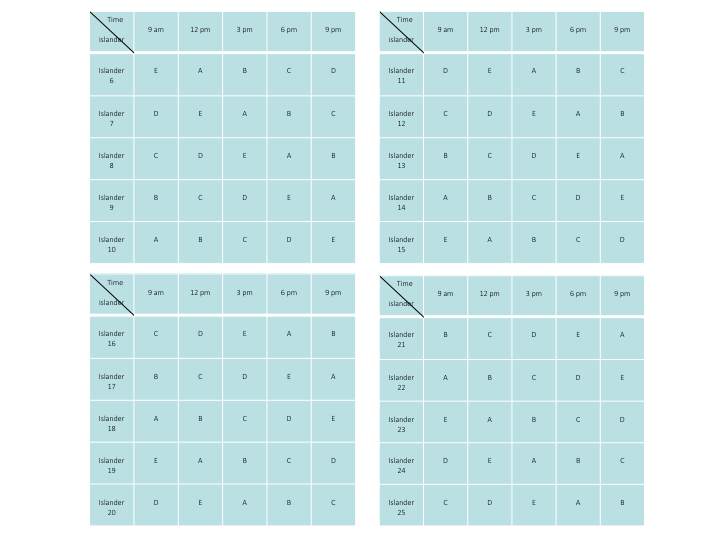
\includegraphics[width=0.98000\textwidth]{Squares.png}
\caption{Latin Square Design - Replicates}
\end{figure}

\begin{itemize}
\tightlist
\item
  \textbf{Held-constant variables}:

  \begin{itemize}
  \tightlist
  \item
    gender: male
  \item
    region: town Macondo
  \item
    age: seniors (age between 65 and 89)
  \end{itemize}
\item
  \textbf{Nuisance factors}:

  \begin{itemize}
  \tightlist
  \item
    individuals: five individuals in each Latin Square
  \item
    time of treatment: 9 am, 12 pm, 3 pm, 6 pm, and 9 pm
  \end{itemize}
\item
  \textbf{Treatment}:

  \begin{itemize}
  \tightlist
  \item
    type of music: no music (A), Classical Music (B), Country Music (C),
    Dance Music (D), or Heavy Metal Music (E)
  \end{itemize}
\item
  \textbf{Replicates}:

  \begin{itemize}
  \tightlist
  \item
    sample size determination: 5 replicates of a 5 x 5 Latin Square
    (i.e., 25 individuals in total)
  \end{itemize}
\end{itemize}

\begin{figure}
\centering
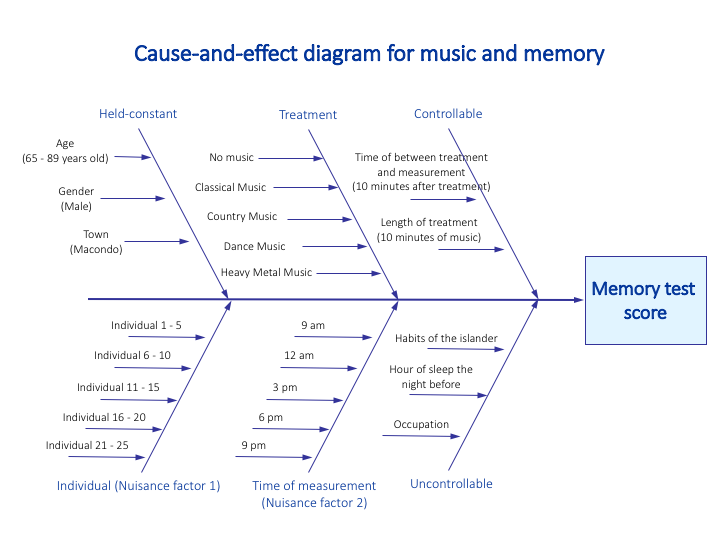
\includegraphics{Diagram.png}
\caption{Cause-and-effect Diagram}
\end{figure}

\begin{itemize}
\tightlist
\item
  \textbf{Random assignment method}:

  \begin{enumerate}
  \def\labelenumi{(\arabic{enumi})}
  \tightlist
  \item
    We assign a number from 1 to 25 to the 25 participants, then
    generate a random sequence (A) of number from 1 to 25 using R
    (\texttt{set.seed(10000)}). Then we generate a random sequence (B)
    of 1 to 5 (\texttt{set.seed(10000)}). We assign the participants
    indexed with the first five number of sequence A to the Latin Square
    replicate indexed with the first number in sequence B; the next five
    in A to the second number in B so on and so forth.
  \item
    We then randomly permute the columns, randomly permute the rows, and
    then assign the treatments to the Latin letters in a random fashion.
    We ensure each treatment occur once in each row and each column.
  \end{enumerate}
\end{itemize}

\subsection{Instruments}\label{instruments}

For this experiment, we use simulated islanders on
\href{http://island.maths.uq.edu.au/index.php}{\texttt{The\ Island}}\footnote{\href{http://island.maths.uq.edu.au}{\texttt{The\ Island:\ http://island.maths.uq.edu.au}}}.
We will use the different genre of music under ``Music'' task to assign
treatment at designated time, and record performance of ``Memory Test
Card''. Realistically, measurement errors are introduced in the study as
the time of measurement cannot be exact (e.g., 9 am sharp). However, we
are allowing small measuring errors since it would not have significant
impact on our final result.

\subsection{Procedure}\label{procedure}

\begin{enumerate}
\def\labelenumi{(\arabic{enumi})}
\tightlist
\item
  For each Latin Square experiment, we first measure the performance of
  ``Memory Test Card'', then wait for 5 minutes.
\item
  Then we assign treatment according to the below diagram; after the
  music treatment finishes, we wait 10 minutes then perform a second
  ``Memory Test Card'' and record the result.
\item
  We replicate the above procedure for all 5 Latin Squares.
\end{enumerate}

\section{Data Analysis}\label{data-analysis}

\subsection{Data Structure}\label{data-structure}

\begin{longtable}[]{@{}llrrlr@{}}
\caption{Structure of data collected}\tabularnewline
\toprule
ID & treatment & before & after & time & difference\tabularnewline
\midrule
\endfirsthead
\toprule
ID & treatment & before & after & time & difference\tabularnewline
\midrule
\endhead
1 & A & 10 & 9 & 9:00 & -1\tabularnewline
1 & E & 10 & 8 & 12:00 & -2\tabularnewline
1 & B & 7 & 9 & 15:00 & 2\tabularnewline
1 & C & 9 & 9 & 18:00 & 0\tabularnewline
1 & D & 6 & 7 & 21:00 & 1\tabularnewline
2 & D & 8 & 7 & 9:00 & -1\tabularnewline
2 & C & 8 & 5 & 12:00 & -3\tabularnewline
2 & E & 9 & 7 & 15:00 & -2\tabularnewline
2 & A & 8 & 9 & 18:00 & 1\tabularnewline
2 & B & 9 & 9 & 21:00 & 0\tabularnewline
\bottomrule
\end{longtable}

\subsection{Statistics of sample}\label{statistics-of-sample}

\textbf{Age distribution: }

Firstly, we took a look at the age distribution of 25 senior male
islanders that we sampled during the experiment:

\begin{figure}
\centering
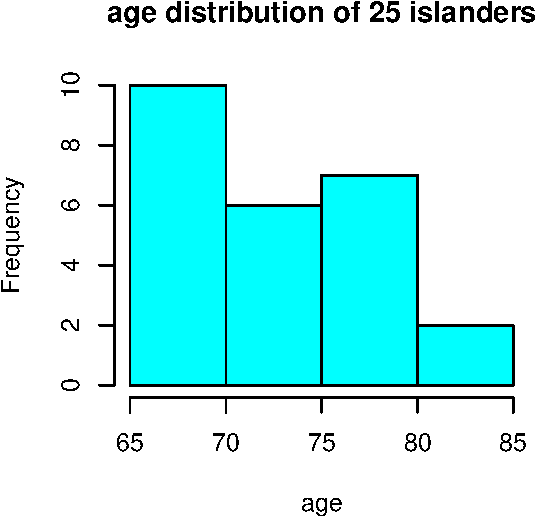
\includegraphics{STATS101B-Project_files/figure-latex/unnamed-chunk-2-1.pdf}
\caption{Age distribution of sample}
\end{figure}

\textbf{Music preference:}

After conducting the experiment on the Island, we also sent out a
post-experiment survey to the selected 25 islanders. The purpose of this
survey is to see which type of music is the islander's favorite, among
all four types of music (classical, country, dance and heavy metal
music).

The result of the survey is as following:

\begin{figure}
\centering
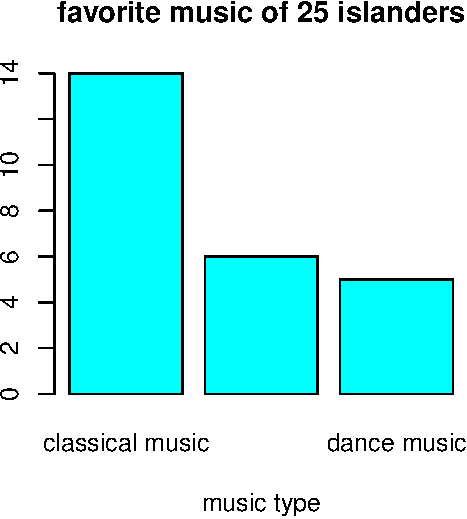
\includegraphics{STATS101B-Project_files/figure-latex/unnamed-chunk-3-1.pdf}
\caption{barplot for results of survey}
\end{figure}

Observation:

\begin{itemize}
\tightlist
\item
  Age distribution: most of the senior male islanders have the age
  between 65 to 80 years old.
\item
  Favorite music type: most of the islanders sampled prefer listening to
  classical music, while a small portion of the islanders prefer country
  and dance music. One important observation is that none of the 25
  islanders we sampled prefer listening to heavy metal music, which may
  be closely connected with results.
\end{itemize}

\subsection{Exploratory Data Analysis
(EDA)}\label{exploratory-data-analysis-eda}

In this section, we did exploratory data analysis by looking at the
boxplots for each Latin Square and the boxplot for all five Latin
Squares combined.

\textbf{Boxplot for each individual Latin Square:}

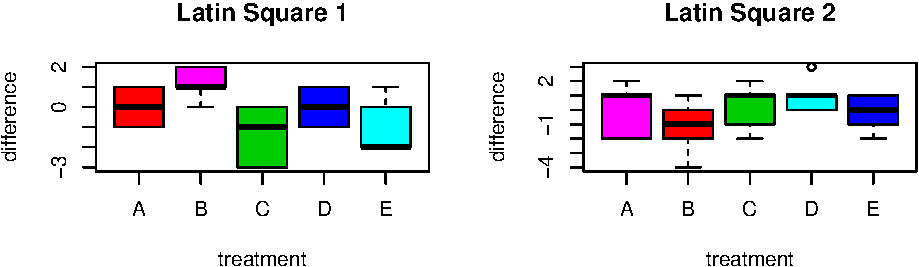
\includegraphics{STATS101B-Project_files/figure-latex/unnamed-chunk-4-1.pdf}

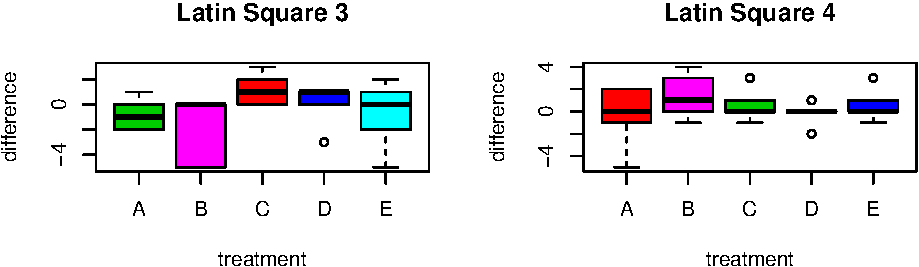
\includegraphics{STATS101B-Project_files/figure-latex/unnamed-chunk-5-1.pdf}

\begin{figure}
\centering
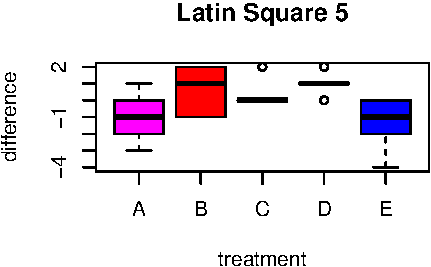
\includegraphics{STATS101B-Project_files/figure-latex/unnamed-chunk-6-1.pdf}
\caption{Boxplots for individual Latin Squares}
\end{figure}

\textbf{Boxplot for all five Latin Squares combined:}

\begin{figure}
\centering
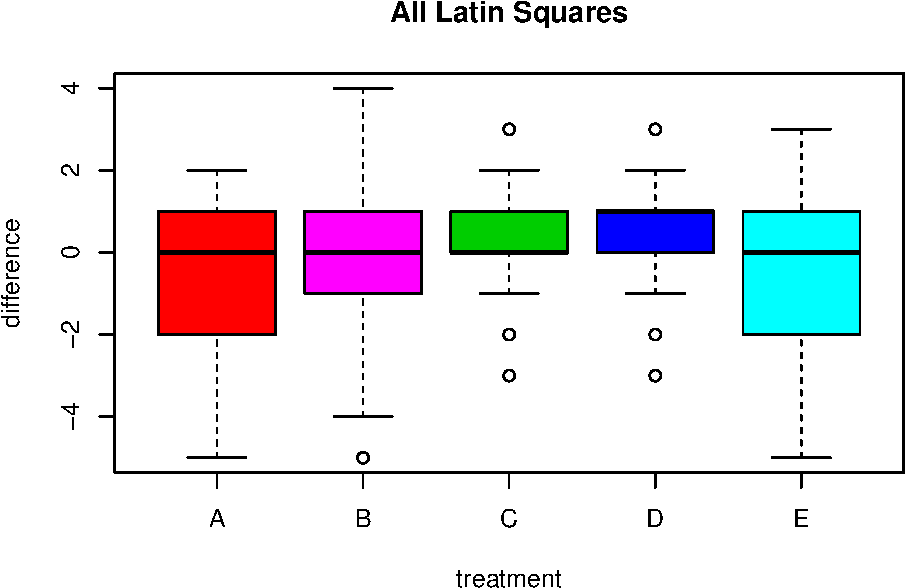
\includegraphics{STATS101B-Project_files/figure-latex/unnamed-chunk-7-1.pdf}
\caption{Boxplot for all five Latin Squares}
\end{figure}

\subsection{Paired t-test}\label{paired-t-test}

We conducted a paired t-test between the memory test score before and
after the treatment.

\begin{longtable}[]{@{}ccccc@{}}
\caption{Paired t-test: \texttt{before} and
\texttt{after}}\tabularnewline
\toprule
\begin{minipage}[b]{0.18\columnwidth}\centering\strut
Test statistic\strut
\end{minipage} & \begin{minipage}[b]{0.06\columnwidth}\centering\strut
df\strut
\end{minipage} & \begin{minipage}[b]{0.10\columnwidth}\centering\strut
P value\strut
\end{minipage} & \begin{minipage}[b]{0.26\columnwidth}\centering\strut
Alternative hypothesis\strut
\end{minipage} & \begin{minipage}[b]{0.26\columnwidth}\centering\strut
mean of the differences\strut
\end{minipage}\tabularnewline
\midrule
\endfirsthead
\toprule
\begin{minipage}[b]{0.18\columnwidth}\centering\strut
Test statistic\strut
\end{minipage} & \begin{minipage}[b]{0.06\columnwidth}\centering\strut
df\strut
\end{minipage} & \begin{minipage}[b]{0.10\columnwidth}\centering\strut
P value\strut
\end{minipage} & \begin{minipage}[b]{0.26\columnwidth}\centering\strut
Alternative hypothesis\strut
\end{minipage} & \begin{minipage}[b]{0.26\columnwidth}\centering\strut
mean of the differences\strut
\end{minipage}\tabularnewline
\midrule
\endhead
\begin{minipage}[t]{0.18\columnwidth}\centering\strut
0.562\strut
\end{minipage} & \begin{minipage}[t]{0.06\columnwidth}\centering\strut
124\strut
\end{minipage} & \begin{minipage}[t]{0.10\columnwidth}\centering\strut
0.5751\strut
\end{minipage} & \begin{minipage}[t]{0.26\columnwidth}\centering\strut
two.sided\strut
\end{minipage} & \begin{minipage}[t]{0.26\columnwidth}\centering\strut
0.088\strut
\end{minipage}\tabularnewline
\bottomrule
\end{longtable}

Based on this result, our observation is that the difference between
before and after the treatment is very small, which indicates that the
overall result may not be very significant.

\subsection{Analysis of Variance
(ANOVA)}\label{analysis-of-variance-anova}

We will conduct an ANOVA test on the results collected. We will first
load the data into R and use \texttt{aov()} function to analyze if there
is any difference among the effects of different genre of music on
memory retention in male aged 65 to 79, among all five 5 x 5 Latin
Squares in data collected.

In this process, we will use paired t-test to determine if there is any
significant difference among the different groups of genres of music and
disregard the interactions between nuisance variables. That is to say,
we will obtain the degrees of freedom, sum of squares and mean sum of
squares for row and column blocks, the treatment, and their
\texttt{F-value} and \texttt{p-value} in the summary statistics.

We divided our analysis of variance (ANOVA) into two sections:

\begin{itemize}
\tightlist
\item
  in the first part, we looked at the ANOVA table for each individual
  Latin Square;
\item
  in the second part, we investigated the ANOVA table for all five Latin
  Squares combined.
\end{itemize}

\textbf{Part 1: ANOVA of five individual Latin Squares:}

\textbf{Latin Square 1:}

\begin{longtable}[]{@{}cccccc@{}}
\caption{Analysis of Variance Table for Latin Square 1}\tabularnewline
\toprule
\begin{minipage}[b]{0.19\columnwidth}\centering\strut
~\strut
\end{minipage} & \begin{minipage}[b]{0.06\columnwidth}\centering\strut
Df\strut
\end{minipage} & \begin{minipage}[b]{0.10\columnwidth}\centering\strut
Sum Sq\strut
\end{minipage} & \begin{minipage}[b]{0.12\columnwidth}\centering\strut
Mean Sq\strut
\end{minipage} & \begin{minipage}[b]{0.12\columnwidth}\centering\strut
F value\strut
\end{minipage} & \begin{minipage}[b]{0.12\columnwidth}\centering\strut
Pr(\textgreater{}F)\strut
\end{minipage}\tabularnewline
\midrule
\endfirsthead
\toprule
\begin{minipage}[b]{0.19\columnwidth}\centering\strut
~\strut
\end{minipage} & \begin{minipage}[b]{0.06\columnwidth}\centering\strut
Df\strut
\end{minipage} & \begin{minipage}[b]{0.10\columnwidth}\centering\strut
Sum Sq\strut
\end{minipage} & \begin{minipage}[b]{0.12\columnwidth}\centering\strut
Mean Sq\strut
\end{minipage} & \begin{minipage}[b]{0.12\columnwidth}\centering\strut
F value\strut
\end{minipage} & \begin{minipage}[b]{0.12\columnwidth}\centering\strut
Pr(\textgreater{}F)\strut
\end{minipage}\tabularnewline
\midrule
\endhead
\begin{minipage}[t]{0.19\columnwidth}\centering\strut
\textbf{treatment}\strut
\end{minipage} & \begin{minipage}[t]{0.06\columnwidth}\centering\strut
4\strut
\end{minipage} & \begin{minipage}[t]{0.10\columnwidth}\centering\strut
20.56\strut
\end{minipage} & \begin{minipage}[t]{0.12\columnwidth}\centering\strut
5.14\strut
\end{minipage} & \begin{minipage}[t]{0.12\columnwidth}\centering\strut
8.965\strut
\end{minipage} & \begin{minipage}[t]{0.12\columnwidth}\centering\strut
0.001365\strut
\end{minipage}\tabularnewline
\begin{minipage}[t]{0.19\columnwidth}\centering\strut
\textbf{ID}\strut
\end{minipage} & \begin{minipage}[t]{0.06\columnwidth}\centering\strut
4\strut
\end{minipage} & \begin{minipage}[t]{0.10\columnwidth}\centering\strut
8.56\strut
\end{minipage} & \begin{minipage}[t]{0.12\columnwidth}\centering\strut
2.14\strut
\end{minipage} & \begin{minipage}[t]{0.12\columnwidth}\centering\strut
3.733\strut
\end{minipage} & \begin{minipage}[t]{0.12\columnwidth}\centering\strut
0.03387\strut
\end{minipage}\tabularnewline
\begin{minipage}[t]{0.19\columnwidth}\centering\strut
\textbf{time}\strut
\end{minipage} & \begin{minipage}[t]{0.06\columnwidth}\centering\strut
4\strut
\end{minipage} & \begin{minipage}[t]{0.10\columnwidth}\centering\strut
12.56\strut
\end{minipage} & \begin{minipage}[t]{0.12\columnwidth}\centering\strut
3.14\strut
\end{minipage} & \begin{minipage}[t]{0.12\columnwidth}\centering\strut
5.477\strut
\end{minipage} & \begin{minipage}[t]{0.12\columnwidth}\centering\strut
0.009582\strut
\end{minipage}\tabularnewline
\begin{minipage}[t]{0.19\columnwidth}\centering\strut
\textbf{Residuals}\strut
\end{minipage} & \begin{minipage}[t]{0.06\columnwidth}\centering\strut
12\strut
\end{minipage} & \begin{minipage}[t]{0.10\columnwidth}\centering\strut
6.88\strut
\end{minipage} & \begin{minipage}[t]{0.12\columnwidth}\centering\strut
0.5733\strut
\end{minipage} & \begin{minipage}[t]{0.12\columnwidth}\centering\strut
NA\strut
\end{minipage} & \begin{minipage}[t]{0.12\columnwidth}\centering\strut
NA\strut
\end{minipage}\tabularnewline
\bottomrule
\end{longtable}

\textbf{Latin Square 2:}

\begin{longtable}[]{@{}cccccc@{}}
\caption{Analysis of Variance Table for Latin Square 2}\tabularnewline
\toprule
\begin{minipage}[b]{0.19\columnwidth}\centering\strut
~\strut
\end{minipage} & \begin{minipage}[b]{0.06\columnwidth}\centering\strut
Df\strut
\end{minipage} & \begin{minipage}[b]{0.10\columnwidth}\centering\strut
Sum Sq\strut
\end{minipage} & \begin{minipage}[b]{0.12\columnwidth}\centering\strut
Mean Sq\strut
\end{minipage} & \begin{minipage}[b]{0.12\columnwidth}\centering\strut
F value\strut
\end{minipage} & \begin{minipage}[b]{0.12\columnwidth}\centering\strut
Pr(\textgreater{}F)\strut
\end{minipage}\tabularnewline
\midrule
\endfirsthead
\toprule
\begin{minipage}[b]{0.19\columnwidth}\centering\strut
~\strut
\end{minipage} & \begin{minipage}[b]{0.06\columnwidth}\centering\strut
Df\strut
\end{minipage} & \begin{minipage}[b]{0.10\columnwidth}\centering\strut
Sum Sq\strut
\end{minipage} & \begin{minipage}[b]{0.12\columnwidth}\centering\strut
Mean Sq\strut
\end{minipage} & \begin{minipage}[b]{0.12\columnwidth}\centering\strut
F value\strut
\end{minipage} & \begin{minipage}[b]{0.12\columnwidth}\centering\strut
Pr(\textgreater{}F)\strut
\end{minipage}\tabularnewline
\midrule
\endhead
\begin{minipage}[t]{0.19\columnwidth}\centering\strut
\textbf{treatment}\strut
\end{minipage} & \begin{minipage}[t]{0.06\columnwidth}\centering\strut
4\strut
\end{minipage} & \begin{minipage}[t]{0.10\columnwidth}\centering\strut
12.56\strut
\end{minipage} & \begin{minipage}[t]{0.12\columnwidth}\centering\strut
3.14\strut
\end{minipage} & \begin{minipage}[t]{0.12\columnwidth}\centering\strut
0.9691\strut
\end{minipage} & \begin{minipage}[t]{0.12\columnwidth}\centering\strut
0.4596\strut
\end{minipage}\tabularnewline
\begin{minipage}[t]{0.19\columnwidth}\centering\strut
\textbf{ID}\strut
\end{minipage} & \begin{minipage}[t]{0.06\columnwidth}\centering\strut
4\strut
\end{minipage} & \begin{minipage}[t]{0.10\columnwidth}\centering\strut
6.56\strut
\end{minipage} & \begin{minipage}[t]{0.12\columnwidth}\centering\strut
1.64\strut
\end{minipage} & \begin{minipage}[t]{0.12\columnwidth}\centering\strut
0.5062\strut
\end{minipage} & \begin{minipage}[t]{0.12\columnwidth}\centering\strut
0.7323\strut
\end{minipage}\tabularnewline
\begin{minipage}[t]{0.19\columnwidth}\centering\strut
\textbf{time}\strut
\end{minipage} & \begin{minipage}[t]{0.06\columnwidth}\centering\strut
4\strut
\end{minipage} & \begin{minipage}[t]{0.10\columnwidth}\centering\strut
6.96\strut
\end{minipage} & \begin{minipage}[t]{0.12\columnwidth}\centering\strut
1.74\strut
\end{minipage} & \begin{minipage}[t]{0.12\columnwidth}\centering\strut
0.537\strut
\end{minipage} & \begin{minipage}[t]{0.12\columnwidth}\centering\strut
0.7115\strut
\end{minipage}\tabularnewline
\begin{minipage}[t]{0.19\columnwidth}\centering\strut
\textbf{Residuals}\strut
\end{minipage} & \begin{minipage}[t]{0.06\columnwidth}\centering\strut
12\strut
\end{minipage} & \begin{minipage}[t]{0.10\columnwidth}\centering\strut
38.88\strut
\end{minipage} & \begin{minipage}[t]{0.12\columnwidth}\centering\strut
3.24\strut
\end{minipage} & \begin{minipage}[t]{0.12\columnwidth}\centering\strut
NA\strut
\end{minipage} & \begin{minipage}[t]{0.12\columnwidth}\centering\strut
NA\strut
\end{minipage}\tabularnewline
\bottomrule
\end{longtable}

\textbf{Latin Square 3:}

\begin{longtable}[]{@{}cccccc@{}}
\caption{Analysis of Variance Table for Latin Square 3}\tabularnewline
\toprule
\begin{minipage}[b]{0.19\columnwidth}\centering\strut
~\strut
\end{minipage} & \begin{minipage}[b]{0.06\columnwidth}\centering\strut
Df\strut
\end{minipage} & \begin{minipage}[b]{0.10\columnwidth}\centering\strut
Sum Sq\strut
\end{minipage} & \begin{minipage}[b]{0.12\columnwidth}\centering\strut
Mean Sq\strut
\end{minipage} & \begin{minipage}[b]{0.12\columnwidth}\centering\strut
F value\strut
\end{minipage} & \begin{minipage}[b]{0.12\columnwidth}\centering\strut
Pr(\textgreater{}F)\strut
\end{minipage}\tabularnewline
\midrule
\endfirsthead
\toprule
\begin{minipage}[b]{0.19\columnwidth}\centering\strut
~\strut
\end{minipage} & \begin{minipage}[b]{0.06\columnwidth}\centering\strut
Df\strut
\end{minipage} & \begin{minipage}[b]{0.10\columnwidth}\centering\strut
Sum Sq\strut
\end{minipage} & \begin{minipage}[b]{0.12\columnwidth}\centering\strut
Mean Sq\strut
\end{minipage} & \begin{minipage}[b]{0.12\columnwidth}\centering\strut
F value\strut
\end{minipage} & \begin{minipage}[b]{0.12\columnwidth}\centering\strut
Pr(\textgreater{}F)\strut
\end{minipage}\tabularnewline
\midrule
\endhead
\begin{minipage}[t]{0.19\columnwidth}\centering\strut
\textbf{treatment}\strut
\end{minipage} & \begin{minipage}[t]{0.06\columnwidth}\centering\strut
4\strut
\end{minipage} & \begin{minipage}[t]{0.10\columnwidth}\centering\strut
27.84\strut
\end{minipage} & \begin{minipage}[t]{0.12\columnwidth}\centering\strut
6.96\strut
\end{minipage} & \begin{minipage}[t]{0.12\columnwidth}\centering\strut
1.772\strut
\end{minipage} & \begin{minipage}[t]{0.12\columnwidth}\centering\strut
0.1992\strut
\end{minipage}\tabularnewline
\begin{minipage}[t]{0.19\columnwidth}\centering\strut
\textbf{ID}\strut
\end{minipage} & \begin{minipage}[t]{0.06\columnwidth}\centering\strut
4\strut
\end{minipage} & \begin{minipage}[t]{0.10\columnwidth}\centering\strut
29.04\strut
\end{minipage} & \begin{minipage}[t]{0.12\columnwidth}\centering\strut
7.26\strut
\end{minipage} & \begin{minipage}[t]{0.12\columnwidth}\centering\strut
1.849\strut
\end{minipage} & \begin{minipage}[t]{0.12\columnwidth}\centering\strut
0.1844\strut
\end{minipage}\tabularnewline
\begin{minipage}[t]{0.19\columnwidth}\centering\strut
\textbf{time}\strut
\end{minipage} & \begin{minipage}[t]{0.06\columnwidth}\centering\strut
4\strut
\end{minipage} & \begin{minipage}[t]{0.10\columnwidth}\centering\strut
10.24\strut
\end{minipage} & \begin{minipage}[t]{0.12\columnwidth}\centering\strut
2.56\strut
\end{minipage} & \begin{minipage}[t]{0.12\columnwidth}\centering\strut
0.652\strut
\end{minipage} & \begin{minipage}[t]{0.12\columnwidth}\centering\strut
0.6365\strut
\end{minipage}\tabularnewline
\begin{minipage}[t]{0.19\columnwidth}\centering\strut
\textbf{Residuals}\strut
\end{minipage} & \begin{minipage}[t]{0.06\columnwidth}\centering\strut
12\strut
\end{minipage} & \begin{minipage}[t]{0.10\columnwidth}\centering\strut
47.12\strut
\end{minipage} & \begin{minipage}[t]{0.12\columnwidth}\centering\strut
3.927\strut
\end{minipage} & \begin{minipage}[t]{0.12\columnwidth}\centering\strut
NA\strut
\end{minipage} & \begin{minipage}[t]{0.12\columnwidth}\centering\strut
NA\strut
\end{minipage}\tabularnewline
\bottomrule
\end{longtable}

\textbf{Latin Square 4:}

\begin{longtable}[]{@{}cccccc@{}}
\caption{Analysis of Variance Table for Latin Square 4}\tabularnewline
\toprule
\begin{minipage}[b]{0.19\columnwidth}\centering\strut
~\strut
\end{minipage} & \begin{minipage}[b]{0.06\columnwidth}\centering\strut
Df\strut
\end{minipage} & \begin{minipage}[b]{0.10\columnwidth}\centering\strut
Sum Sq\strut
\end{minipage} & \begin{minipage}[b]{0.12\columnwidth}\centering\strut
Mean Sq\strut
\end{minipage} & \begin{minipage}[b]{0.12\columnwidth}\centering\strut
F value\strut
\end{minipage} & \begin{minipage}[b]{0.12\columnwidth}\centering\strut
Pr(\textgreater{}F)\strut
\end{minipage}\tabularnewline
\midrule
\endfirsthead
\toprule
\begin{minipage}[b]{0.19\columnwidth}\centering\strut
~\strut
\end{minipage} & \begin{minipage}[b]{0.06\columnwidth}\centering\strut
Df\strut
\end{minipage} & \begin{minipage}[b]{0.10\columnwidth}\centering\strut
Sum Sq\strut
\end{minipage} & \begin{minipage}[b]{0.12\columnwidth}\centering\strut
Mean Sq\strut
\end{minipage} & \begin{minipage}[b]{0.12\columnwidth}\centering\strut
F value\strut
\end{minipage} & \begin{minipage}[b]{0.12\columnwidth}\centering\strut
Pr(\textgreater{}F)\strut
\end{minipage}\tabularnewline
\midrule
\endhead
\begin{minipage}[t]{0.19\columnwidth}\centering\strut
\textbf{treatment}\strut
\end{minipage} & \begin{minipage}[t]{0.06\columnwidth}\centering\strut
4\strut
\end{minipage} & \begin{minipage}[t]{0.10\columnwidth}\centering\strut
10.4\strut
\end{minipage} & \begin{minipage}[t]{0.12\columnwidth}\centering\strut
2.6\strut
\end{minipage} & \begin{minipage}[t]{0.12\columnwidth}\centering\strut
1.04\strut
\end{minipage} & \begin{minipage}[t]{0.12\columnwidth}\centering\strut
0.4266\strut
\end{minipage}\tabularnewline
\begin{minipage}[t]{0.19\columnwidth}\centering\strut
\textbf{ID}\strut
\end{minipage} & \begin{minipage}[t]{0.06\columnwidth}\centering\strut
4\strut
\end{minipage} & \begin{minipage}[t]{0.10\columnwidth}\centering\strut
10.4\strut
\end{minipage} & \begin{minipage}[t]{0.12\columnwidth}\centering\strut
2.6\strut
\end{minipage} & \begin{minipage}[t]{0.12\columnwidth}\centering\strut
1.04\strut
\end{minipage} & \begin{minipage}[t]{0.12\columnwidth}\centering\strut
0.4266\strut
\end{minipage}\tabularnewline
\begin{minipage}[t]{0.19\columnwidth}\centering\strut
\textbf{time}\strut
\end{minipage} & \begin{minipage}[t]{0.06\columnwidth}\centering\strut
4\strut
\end{minipage} & \begin{minipage}[t]{0.10\columnwidth}\centering\strut
33.2\strut
\end{minipage} & \begin{minipage}[t]{0.12\columnwidth}\centering\strut
8.3\strut
\end{minipage} & \begin{minipage}[t]{0.12\columnwidth}\centering\strut
3.32\strut
\end{minipage} & \begin{minipage}[t]{0.12\columnwidth}\centering\strut
0.0475\strut
\end{minipage}\tabularnewline
\begin{minipage}[t]{0.19\columnwidth}\centering\strut
\textbf{Residuals}\strut
\end{minipage} & \begin{minipage}[t]{0.06\columnwidth}\centering\strut
12\strut
\end{minipage} & \begin{minipage}[t]{0.10\columnwidth}\centering\strut
30\strut
\end{minipage} & \begin{minipage}[t]{0.12\columnwidth}\centering\strut
2.5\strut
\end{minipage} & \begin{minipage}[t]{0.12\columnwidth}\centering\strut
NA\strut
\end{minipage} & \begin{minipage}[t]{0.12\columnwidth}\centering\strut
NA\strut
\end{minipage}\tabularnewline
\bottomrule
\end{longtable}

\textbf{Latin Square 5:}

\begin{longtable}[]{@{}cccccc@{}}
\caption{Analysis of Variance Table for Latin Square 5}\tabularnewline
\toprule
\begin{minipage}[b]{0.19\columnwidth}\centering\strut
~\strut
\end{minipage} & \begin{minipage}[b]{0.06\columnwidth}\centering\strut
Df\strut
\end{minipage} & \begin{minipage}[b]{0.10\columnwidth}\centering\strut
Sum Sq\strut
\end{minipage} & \begin{minipage}[b]{0.12\columnwidth}\centering\strut
Mean Sq\strut
\end{minipage} & \begin{minipage}[b]{0.12\columnwidth}\centering\strut
F value\strut
\end{minipage} & \begin{minipage}[b]{0.12\columnwidth}\centering\strut
Pr(\textgreater{}F)\strut
\end{minipage}\tabularnewline
\midrule
\endfirsthead
\toprule
\begin{minipage}[b]{0.19\columnwidth}\centering\strut
~\strut
\end{minipage} & \begin{minipage}[b]{0.06\columnwidth}\centering\strut
Df\strut
\end{minipage} & \begin{minipage}[b]{0.10\columnwidth}\centering\strut
Sum Sq\strut
\end{minipage} & \begin{minipage}[b]{0.12\columnwidth}\centering\strut
Mean Sq\strut
\end{minipage} & \begin{minipage}[b]{0.12\columnwidth}\centering\strut
F value\strut
\end{minipage} & \begin{minipage}[b]{0.12\columnwidth}\centering\strut
Pr(\textgreater{}F)\strut
\end{minipage}\tabularnewline
\midrule
\endhead
\begin{minipage}[t]{0.19\columnwidth}\centering\strut
\textbf{treatment}\strut
\end{minipage} & \begin{minipage}[t]{0.06\columnwidth}\centering\strut
4\strut
\end{minipage} & \begin{minipage}[t]{0.10\columnwidth}\centering\strut
22.24\strut
\end{minipage} & \begin{minipage}[t]{0.12\columnwidth}\centering\strut
5.56\strut
\end{minipage} & \begin{minipage}[t]{0.12\columnwidth}\centering\strut
4.088\strut
\end{minipage} & \begin{minipage}[t]{0.12\columnwidth}\centering\strut
0.02564\strut
\end{minipage}\tabularnewline
\begin{minipage}[t]{0.19\columnwidth}\centering\strut
\textbf{ID}\strut
\end{minipage} & \begin{minipage}[t]{0.06\columnwidth}\centering\strut
4\strut
\end{minipage} & \begin{minipage}[t]{0.10\columnwidth}\centering\strut
5.84\strut
\end{minipage} & \begin{minipage}[t]{0.12\columnwidth}\centering\strut
1.46\strut
\end{minipage} & \begin{minipage}[t]{0.12\columnwidth}\centering\strut
1.074\strut
\end{minipage} & \begin{minipage}[t]{0.12\columnwidth}\centering\strut
0.4118\strut
\end{minipage}\tabularnewline
\begin{minipage}[t]{0.19\columnwidth}\centering\strut
\textbf{time}\strut
\end{minipage} & \begin{minipage}[t]{0.06\columnwidth}\centering\strut
4\strut
\end{minipage} & \begin{minipage}[t]{0.10\columnwidth}\centering\strut
13.44\strut
\end{minipage} & \begin{minipage}[t]{0.12\columnwidth}\centering\strut
3.36\strut
\end{minipage} & \begin{minipage}[t]{0.12\columnwidth}\centering\strut
2.471\strut
\end{minipage} & \begin{minipage}[t]{0.12\columnwidth}\centering\strut
0.1009\strut
\end{minipage}\tabularnewline
\begin{minipage}[t]{0.19\columnwidth}\centering\strut
\textbf{Residuals}\strut
\end{minipage} & \begin{minipage}[t]{0.06\columnwidth}\centering\strut
12\strut
\end{minipage} & \begin{minipage}[t]{0.10\columnwidth}\centering\strut
16.32\strut
\end{minipage} & \begin{minipage}[t]{0.12\columnwidth}\centering\strut
1.36\strut
\end{minipage} & \begin{minipage}[t]{0.12\columnwidth}\centering\strut
NA\strut
\end{minipage} & \begin{minipage}[t]{0.12\columnwidth}\centering\strut
NA\strut
\end{minipage}\tabularnewline
\bottomrule
\end{longtable}

\textbf{Part II: ANOVA for all five Latin Squares}:

\textbf{All five Latin Squares:}

\begin{longtable}[]{@{}cccccc@{}}
\caption{Analysis of Variance Table for five Latin
Squares}\tabularnewline
\toprule
\begin{minipage}[b]{0.19\columnwidth}\centering\strut
~\strut
\end{minipage} & \begin{minipage}[b]{0.06\columnwidth}\centering\strut
Df\strut
\end{minipage} & \begin{minipage}[b]{0.10\columnwidth}\centering\strut
Sum Sq\strut
\end{minipage} & \begin{minipage}[b]{0.12\columnwidth}\centering\strut
Mean Sq\strut
\end{minipage} & \begin{minipage}[b]{0.12\columnwidth}\centering\strut
F value\strut
\end{minipage} & \begin{minipage}[b]{0.12\columnwidth}\centering\strut
Pr(\textgreater{}F)\strut
\end{minipage}\tabularnewline
\midrule
\endfirsthead
\toprule
\begin{minipage}[b]{0.19\columnwidth}\centering\strut
~\strut
\end{minipage} & \begin{minipage}[b]{0.06\columnwidth}\centering\strut
Df\strut
\end{minipage} & \begin{minipage}[b]{0.10\columnwidth}\centering\strut
Sum Sq\strut
\end{minipage} & \begin{minipage}[b]{0.12\columnwidth}\centering\strut
Mean Sq\strut
\end{minipage} & \begin{minipage}[b]{0.12\columnwidth}\centering\strut
F value\strut
\end{minipage} & \begin{minipage}[b]{0.12\columnwidth}\centering\strut
Pr(\textgreater{}F)\strut
\end{minipage}\tabularnewline
\midrule
\endhead
\begin{minipage}[t]{0.19\columnwidth}\centering\strut
\textbf{treatment}\strut
\end{minipage} & \begin{minipage}[t]{0.06\columnwidth}\centering\strut
4\strut
\end{minipage} & \begin{minipage}[t]{0.10\columnwidth}\centering\strut
15.95\strut
\end{minipage} & \begin{minipage}[t]{0.12\columnwidth}\centering\strut
3.988\strut
\end{minipage} & \begin{minipage}[t]{0.12\columnwidth}\centering\strut
1.277\strut
\end{minipage} & \begin{minipage}[t]{0.12\columnwidth}\centering\strut
0.2849\strut
\end{minipage}\tabularnewline
\begin{minipage}[t]{0.19\columnwidth}\centering\strut
\textbf{ID}\strut
\end{minipage} & \begin{minipage}[t]{0.06\columnwidth}\centering\strut
24\strut
\end{minipage} & \begin{minipage}[t]{0.10\columnwidth}\centering\strut
70.83\strut
\end{minipage} & \begin{minipage}[t]{0.12\columnwidth}\centering\strut
2.951\strut
\end{minipage} & \begin{minipage}[t]{0.12\columnwidth}\centering\strut
0.9448\strut
\end{minipage} & \begin{minipage}[t]{0.12\columnwidth}\centering\strut
0.5436\strut
\end{minipage}\tabularnewline
\begin{minipage}[t]{0.19\columnwidth}\centering\strut
\textbf{time}\strut
\end{minipage} & \begin{minipage}[t]{0.06\columnwidth}\centering\strut
4\strut
\end{minipage} & \begin{minipage}[t]{0.10\columnwidth}\centering\strut
5.872\strut
\end{minipage} & \begin{minipage}[t]{0.12\columnwidth}\centering\strut
1.468\strut
\end{minipage} & \begin{minipage}[t]{0.12\columnwidth}\centering\strut
0.47\strut
\end{minipage} & \begin{minipage}[t]{0.12\columnwidth}\centering\strut
0.7576\strut
\end{minipage}\tabularnewline
\begin{minipage}[t]{0.19\columnwidth}\centering\strut
\textbf{Residuals}\strut
\end{minipage} & \begin{minipage}[t]{0.06\columnwidth}\centering\strut
92\strut
\end{minipage} & \begin{minipage}[t]{0.10\columnwidth}\centering\strut
287.4\strut
\end{minipage} & \begin{minipage}[t]{0.12\columnwidth}\centering\strut
3.124\strut
\end{minipage} & \begin{minipage}[t]{0.12\columnwidth}\centering\strut
NA\strut
\end{minipage} & \begin{minipage}[t]{0.12\columnwidth}\centering\strut
NA\strut
\end{minipage}\tabularnewline
\bottomrule
\end{longtable}

Based on the ANOVA table obtained above, we observe that:

\begin{itemize}
\tightlist
\item
  Among all five individual Latin Squares, music treatment in Latin
  Square 1 and Latin Square 5 have significant effects on improving
  memory test score.
\item
  However, music treatment is not significant when we combine all five
  Latin Squares together.
\end{itemize}

To explore more about which music treatment is more helpful for
improving memory test score on islanders, we conducted multiple groups
comparision tests on Latin Square 1 and Latin Square 5.

\subsection{Multiple groups
comparison}\label{multiple-groups-comparison}

From the last section, we observe that music treatment is indeed
significant in Latin Square 1 and 5. To see which music plays a more
important role in improving the memory test score, we did multiple
groups comparison on each of the two squares, using \texttt{Tukey\ HSD}
method.

\textbf{Multiple groups comparison for Latin Square 1:}

\begin{figure}
\centering
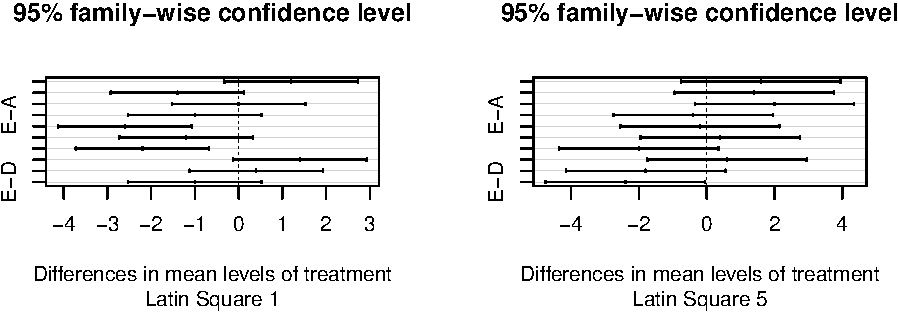
\includegraphics{STATS101B-Project_files/figure-latex/unnamed-chunk-10-1.pdf}
\caption{Multiple groups comparison on Latin Square 1 and 5}
\end{figure}

\textbf{Multiple groups comparison for Latin Square 5:}

Based on the multiple groups comparison, we observe that:

\begin{itemize}
\tightlist
\item
  In Latin Square 1:
\item
  In Latin Square 2:
\end{itemize}

\subsection{Model assumption checking}\label{model-assumption-checking}

\textbf{Model}:

\[y_{ijk} = \mu + \alpha_{i} + \beta_{j} + \gamma_{k} + \epsilon_{ijk},\ where\  i, j, k = 1, 2, 3, 4, 5\]

\textbf{Assumption checking:}

\begin{figure}
\centering
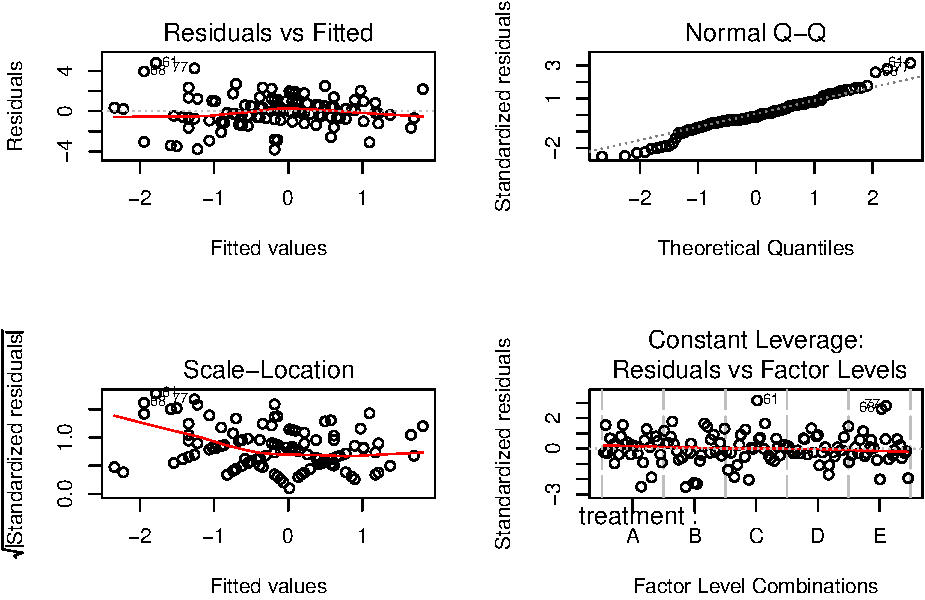
\includegraphics{STATS101B-Project_files/figure-latex/unnamed-chunk-11-1.pdf}
\caption{Diagnostics plots for model difference \textasciitilde{}
treatment + ID + time}
\end{figure}

\begin{itemize}
\tightlist
\item
  Based on the residuals vs.~fitted values plot, we observe that there
  is no certain pattern in the graph, and the average value of error
  terms is mostly around zero. This indicates that the assumption of
  independent error terms with average value of zero is satisfied.
\item
  Based on the normal QQ-plot, we observe that most of the data points
  are around the 45-degree line through the origin. This indicates that
  the assumption of normally distributed error terms is mostly
  satisfied.
\item
  Based on the \(\sqrt{standardized\ residuals}\) vs.~fitted values
  plot, we observe that there is a slightly decreasing trend in the
  value of \(\sqrt{standardized\ residuals}\). This indicates that the
  assumption of constant variance of error terms is slightly violated.
\end{itemize}

\section{Conclusion}\label{conclusion}

To be finished.

\section{Discussion}\label{discussion}

\begin{itemize}
\tightlist
\item
  Since we choose to sample senior islanders in the experiment, we
  consider sampling senior female islanders in the future to have
  further investigation on whether music has effects on memory.
\item
  Based on the post-experiment survey, we discovered that most of the
  senior islanders prefer listening to classical and country music. This
  provides motivation for further studies on the relation between
  favorite type of music, music treatment, and memory test score.
\end{itemize}

\section{References}\label{references}

\subsection{Journal References}\label{journal-references}

\begin{itemize}
\tightlist
\item
  \href{https://www.scientificamerican.com/article/music-and-the-brain-2006-09/}{\texttt{Music\ And\ The\ Brain}},
  Norman M. Weinberger. \emph{Scientific American}, September 1, 2006.
\item
  \href{https://med.stanford.edu/news/all-news/2007/07/music-moves-brain-to-pay-attention-stanford-study-finds.html}{\texttt{Music\ Moves\ Brain\ to\ Pay\ Attention}},
  Mitzi Baker. \emph{Stanford Medicine News Center}, August 1, 2007.
\item
  \href{https://www.cnn.com/2013/04/15/health/brain-music-research/index.html}{\texttt{This\ is\ Your\ Brain\ on\ Music}},
  Elizabeth Landau. \emph{CNN}, January 23, 2018.
\item
  \href{https://www.health.harvard.edu/staying-healthy/music-and-health}{\texttt{Music\ and\ health}},
  \emph{Harvard Medical School}, July 2011.
\item
  \href{https://www.encyclopedia.com/psychology/encyclopedias-almanacs-transcripts-and-maps/individual-differences-learning-and-memory}{\texttt{Individual\ Differences\ in\ Learning\ and\ Memory}}.
  \emph{Encyclopedia}, 2014.
\end{itemize}

\subsection{Publication References}\label{publication-references}

\begin{itemize}
\tightlist
\item
  \href{https://search.proquest.com/docview/1701283142?pq-origsite=summon\&accountid=14512}{\texttt{A\ neuropsychological\ investigation\ of\ music,\ emotion,\ and\ autobiographical\ memory}},
  Belfi, Amy Meredith. \emph{University of Iowa}, 2015.
\item
  \href{https://search.proquest.com/docview/304910597?pq-origsite=summon\&accountid=14512}{\texttt{Music\ in\ the\ brain:\ Differences\ between\ musicians\ and\ non-musicians}},
  Orlando, Julie. \emph{University of Northern British Columbia
  (Canada)}, 2006.
\item
  \href{https://search.proquest.com/docview/2083960675?accountid=14512}{\texttt{Music\ for\ the\ Mind:\ A\ Study\ Into\ Musical\ Preferences,\ Personality\ Traits\ and\ Memory\ Retention}},
  Rogers, Rhiannon. \emph{Western Sydney University (Australia)}, 2018.
\item
  \href{https://search.proquest.com/docview/305228684?pq-origsite=summon\&accountid=14512}{\texttt{Music\ and\ cognitive\ abilities:\ A\ look\ at\ the\ Mozart\ Effect}},
  Bressler, Randy A. \emph{The Chicago School of Professional
  Psychology}, 2003.
\item
  \href{https://www.sciencedirect.com/science/article/pii/S1878875010001129}{\texttt{Music\ and\ the\ Brain}},
  Edward R. Laws, Jr. \emph{Harvard University}, 2010.
\item
  \href{https://scholar.utc.edu/cgi/viewcontent.cgi?article=1214\&context=mps}{\texttt{The\ effect\ of\ music\ genre\ on\ a\ memory\ task}},
  Bugter, Darragh \& Carden, Randy. \emph{Trevecca Nazarene University},
  2012.
\item
  \href{http://memory.psych.upenn.edu/files/pubs/HealEtal14.pdf}{\texttt{Individual\ Differences\ in\ Memory\ Search\ and\ Their\ Relation\ to\ Intelligence}},
  M. Karl Healey. \emph{University of Pennsylvania}, 2014.
\item
  \href{https://journals.sagepub.com/doi/10.1080/14640747008401939}{\texttt{Memory\ and\ time\ of\ day}},
  A. D. Baddeley, J. E. Hatter, Denise Scott \& Aileen Snashall.
  \emph{Quarterly Journal of Experimental Psychology}, 1970.
\item
  \href{https://scholar.utc.edu/mps/vol17/iss2/14}{\texttt{The\ effect\ of\ music\ genre\ on\ a\ memory\ task}},
  Bugter, Darragh and Carden, Randy.\emph{Modern Psychological Studies,
  Vol. 17, No.2, Article 14}, 2012.
\item
  \href{https://www.frontiersin.org/articles/10.3389/fnhum.2014.00395/full}{\texttt{Music\ mnemonics\ aid\ Verbal\ Memory\ and\ Induce\ Learning\ –\ Related\ Brain\ Plasticity\ in\ Multiple\ Sclerosis}},
  Thaut, Michael \& Peterson, David \& C McIntosh, Gerald \& Hömberg,
  Volker. \emph{Frontiers in human neuroscience}, 2014.
\item
  \href{https://journals.sagepub.com/doi/10.2466/pms.1998.86.3.835}{\texttt{Key\ Components\ of\ the\ Mozart\ Effect}},
  Frances H. Rauscher \& Gordon L. Shaw. \emph{University of Wiscomin,
  Osbkosb} \& \emph{University of California, Irvine}, 1998.
\end{itemize}


\end{document}
